\documentclass{article}

\usepackage{amsmath}
\usepackage{amssymb}
\usepackage{mathtools}
\usepackage{fullpage}
\usepackage{enumerate}
\usepackage{graphicx}

\title{Computer Science 577 Notes \\ Introduction to Algorithms}
\author{Mendel C. Mayr}
\date{\today}

\begin{document}
	\maketitle
	\vspace{10pt}
	\begin{center}
		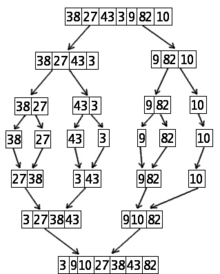
\includegraphics[width = 2.7in]{mergesort.png}
		\end{center}
	\vspace{12pt}
	\tableofcontents
	\clearpage

	\section{Recurrence Relations}
		\subsection{Recursive Analysis of Insertion and Merge Sort}
			Insertion sort: let $M(n)$ be the comparisons required to sort a list of size $n$ \\
			Analysis: note that $M(1) = 0$ and $M(n) = M(n - 1) + n$ for $n > 1$
			\begin{enumerate}[(i)]
				\item $M(n) = M(n - 1) + n$
				\item $M(n) = M(n - 2) + n + (n - 1)\:...$
				\item $M(n) = M(n - k) + n + (n - 1) +\:...\:+ (n - k + 1)$
				\item Let $k = n - 1$, $M(n) = M(1) + n(n - n + 1) + \sum_{i = 1}^{n - 1}i$
				\item $M(n) = 0 + n + (n - 1)(n - 2)/2 \approx n^2/2$
				\end{enumerate}
			Merge sort: let $M(n)$ be the comparison required to sort a list of size $n$ \\
			\\
			Analysis: for simplcity, consider only $n$ such that $n = 2^a$ for some integer $a$ \\
			Note that $M(1) = 0$ and $M(n) = 2M(n/2) + n$ for $n > 1$
			\begin{enumerate}[(i)]
			 	\item $M(n) = 2M(n/2) + n$
			 	\item $M(n) = 2M(n/4) + n + (n/2)$
			 	\item $M(n) = 2M(n/2^k) + n + (n/2) +\:....\:+ (n/2^{k - 1})$
			 	\item Let $k = a$, $2M(1) + \sum_{i = 1}^{k - 1} n/2^i$ (unclarified point)
			 	\item Mergsort is $O(n \log n)$
			 	\end{enumerate}
		\subsection{Recursive Linear Selection}
			Recursive linear selection algorithm: given $x_1, x_2, ..., x_n$ distinct keys, find $x_k$ (i.e. the $k$th smallest element) without using sorting \\
			Note: the rank of an element (i.e. the number of keys greater than it) can be found in linear time \\
			Linear selection algorithm is as folows:
			\begin{enumerate}[(i)]
				\item Remove keys of known rank, to make $n = 5 (mod 10)$
				\item Divide elements into groups of 5, denoted $S[i]$ for $i$ from $1$ to $n/5$
				\item Recursively find the median of each group, denoted $x[i]$
				\item Let $M^*$ be the median of the set $x[i]$ for $i$ from $1$ to $n/5$
				\item Divide keys into groups of keys less than (call this $L$), equal to, or greater than (call this $R$) $M^*$
				\item Recursiveley process one of $L$ or $R$
				\end{enumerate}
			Analysis: Note that steps 1, 2, and 5 are $O(n)$, so the number of computations for this algorithm, $T(n) = T(n/5) + T(7n/10) + O(n)$ \\
			Guessing and proving: supposed that $T(n) = O(n)$, which can be proven via strong induction, i.e. $T(n) < An$ for some constant $A$ for all $n$ \\
			Recall that strong induction relies on proving two claims:
			\begin{enumerate}[(i)]
				\item The statement holds for all $n \geq 1$, $\forall n \leq n_0$ (base case)
				\item If the statmenet holds for all $i < n$, it holds for $n$
				\end{enumerate}
			Proof of second part of strong inductive proof:
			\begin{enumerate}[(i)]
				\item Suppose that $T(n) = O(n)$ for $i < n$
				\item We seek and $A$ such that $A(n/5) + A(7n/10) + cn \leq An$
				\item Thus, $A \geq 10c$ is sufficient for this part
				\end{enumerate}
			Proof of first part of strong inductive proof: need $A$ such that $n(n - 1)/2 \leq An$ for $1 \leq n \leq 10$ \\
			So $A \geq 9/10$ is sufficient for this part \\
			\\
			Conclusion: $A = max\{9/2, 10c\}$ will suffice to show that $T(n) = O(n)$ 
		\subsection{Recursive Quadratic Closest-Pair}
			Recursive quadratic algorithm: find closest pair of points
			\begin{enumerate}[i]
				\item (Supposing that $n = 2^k$) into 2 equal groups, denoted $L$ and $R$
				\item Recurisvely find the closest pair in $L$ and $R$
				\item Report closest pair form testing elements of $L$ against elements of $R$
				\item Report best pair out of those from steps (ii) and (iii)
				\end{enumerate}
			Analysis: $T(n) = 2(T/n) + O(n^2)$ for $n = 2^k \geq 4$, $T(2) = 1$ \\
			The $O(n^2)$ in the recursive case comes from step (iii) \\
			\\
			Consider the recursion tree, which is full binary tree: at the first level, the problem size is $n, n/2, n/4, ...$ at the first, second, third, etc. levels. Thus, the number of computations required is $n^2$ at the first level, $2(n/2)^2 = n^2/2$ at the second level, $2(n/4)^2 = n^2/4$ at the third, etc. \\
			\\
			Thus, the maximum number of computations is $\sum_{k = 1}^\infty n^2/2^k = 2n^2$, thus $T(n) = O(n^2)$
		\subsection{Divide and Conquer Recurrences and Master Theorem}
			Master theorem: if $T(n) = aT(n/b) + O(n^d)$ for some constants $a > 0, b > 1$, and $d \geq 0$, then:
			\begin{enumerate}[(i)]
				\item $T(n) = O(n^d)$ if $d > \log_b a$
				\item $T(n) = O(n^d \log n)$ if $d = \log_b a$
				\item $T(n) = O(n^{\log_b a})$ if $d < \log_b a$
				\end{enumerate}
			Proof: consider the recursion tree for such a problem \\
			Notice that $a$ is the branching factor of the problem. At the $i$th level (starting at index 0), there are $a^i$ subproblems of size $n/b^i$. which means the computation that must be done at that level is $a^iO((n/b^i)^d)$ \\
			The number of levels in the recusion tree is $k = \log_b n$ \\
			As such: $T(n) = \sum_{i = 0}^k a_iO((n/b^i)^d) = O(n^d)\sum_{i = 0}^k(a/b^d)^i$. Now consider the cases
			\begin{enumerate}[(i)]
				\item If $d > \log_b a$, then $a/b^d < 1$ \\
				$\sum_{i = 0}^\infty (a/b^d)^i < \infty$ (i.e. series converges) \\
				$\sum_{i = 0}^\infty (a/b^d)^i = O(1)$, so $T(n) = O(n^d)$
				\item If $d = \log_b a$, then $a/b^d = 1$ \\
				$\sum_{i = 0}^k (a/b^d)^i = \sum_{i = 0}^k 1 = k + 1$, since $k = \log_b n = \log n/\log b = O(\log n)$ \\
				Therefore, $T(n) = O(n^d\log n)$
				\item If $d < \log_b a$, then $a/b^d > 1$ \\
				$\sum_{i = 0}^k (a/b^d)^i = O((a/b^d)^k)$, so $T(n) = O(n^d)O(a^k)/b^{dk}$ \\
				Since $k = \log_b n, n = b^k$, $T(n) = O(n^d)O(a^k)/n^d = O(a^k)$ \\
				$a^k = a^{\log_b n} = n^{\log_b a}$, so $T(n) = O(n^{\log_b a})$
				\end{enumerate}
		\subsection{Asymptotics}
			Notation for asymptotics:
			\begin{enumerate}[(i)]
				\item $f$ and $g$ are real value functions on $x \geq 0$. $f(x)$, $g(x) \geq 0$ for sufficiently large $x$ \\
				Sufficently large: $\exists x_0 > 0$ such that $f(x) \geq 0$ when $x \geq x_0$
				\item $f = O(g)$ means that for some $c > 0$ and $x_0 > 0$, $f(x) \leq cg(x)$ for al $x \geq x_0$
				\item $f = \Omega(g)$ means that for some $c > 0$ and $x_0 \geq 0$, $f(x) \geq xg(x)$ for all $x \geq x_0$ \\
				This is equivalent to saying that $g = O(f)$
				\item $f = \Theta(g)$ means that $f = O(g)$ and $f = \Theta(g)$
				\end{enumerate}
			Demonstrating that $f = O(g)$ can be done algebraically, or via L'Hopital's rule \\
			\\
			Additional definitions:
			\begin{enumerate}[(i)]
				\item $f = o(g)$ means $\lim_{x \to \infty} f(x)/g(x) = 0$
				\item $f \sim g$ means $\lim_{x \to \infty} f(x)/g(x) = 1$
				\end{enumerate}
			Polynomial growth: $f$ is polynomially bounded if $f(x) = O(x^k)$ for some $k > 0$, (efficiently computable) \\
			Exponential growth: $f$ is exponential growth if $f(x) = O(\alpha^x)$ for some $\alpha > 1$
		\subsection{Arithmetic Algorithms}
			Addition: elementary (i.e. sum and carry bits), adding two $n$-bit numbers has $O(n)$ complexity \\
			Subtraction: inverse of addition, similarly requires $O(n)$ times \\
			Multiplication: elementary algorithm requires $O(n)$ times
			\\
			There exists an $O(n^a)$ algorithm for multiplication, where $a < 2$: \\
			For multiplying $n$-bit numbers, where $n = 2^k$:
			\begin{enumerate}[(i)]
				\item $x = 2^{n/2}x_1 + x_0$, $y = 2^{n/2}y_1 + y_0$
				\item $xy = 2^nx_1y_1 + 2^{n/2}(x_1y_0 + x_0y_1) + x_0y_0$
				\item Let $a = x_1y_1$, $c = x_0y_0$, $d = (x_1 + x_2)(y_1 + y_2)$
				\item Let $b = x_1y_0 + x_oy_1$, note that $b = D - A - C$
				\end{enumerate}
			Analysis: let $k(n)$ be the complexity of this algorithm \\
			$k(n) = 3k(n/2) + O(n)$ when $n > 1$, $K(n) = O(1)$ when $n = 1$ \\
			By the master theorem: $k(n) = O(n^{\log_2 3}) \approx O(n^{1.59})$ \\
			\\
			Using Newton interation, division reducible to multiplication: similar complexity \\
			Open question: does there exist $O(n)$ algorithm for multiplication \\
			\\
			Matrix multiplication: let $A = (a_{i, j}), B = (b_{i ,j})$ for $1 \leq i, j \leq n$ \\
			Then $C = (c_{i, j})$, where $c_{i, j} = \sum_{k = 1}^n a_{i, k}n_{k, j}$
		\clearpage
		
	\appendix

	\section{Review of Basic Mathematical Concepts}
		\subsection{Properties of Logarithms}
			Change of base: $\log_a x = \log_b x/\log_b a$ \\
			Basic properties:
			\begin{enumerate}[(i)]
				\item $\log_a(uv) = \log_a u + \log_a v$
				\item $\log_a(u / v) = \log_a u - \log_a v$
				\item $\log_a u^n = n \log_a u$
				\end{enumerate}



	\end{document}